\documentclass[11pt]{article}
\usepackage[margin=1in]{geometry}
\usepackage{amsmath,amssymb,amsthm}
\usepackage{algorithm}
\usepackage{algpseudocode}
\usepackage{booktabs}
\usepackage{hyperref}
\usepackage{tikz}
\usetikzlibrary{positioning,shapes.geometric,shapes.misc}

\newtheorem{definition}{Definition}
\newtheorem{theorem}{Theorem}
\newtheorem{example}{Example}

\title{ApproxLP: Approximate Credal Network Inference\\via Iterative Linearization}
\author{IBM Research}
\date{}

\begin{document}
\maketitle

\begin{abstract}
ApproxLP is an approximate inference algorithm for credal networks that reformulates
the marginal inference problem as a multilinear program and solves it via iterative
linearization (coordinate descent). At each step, all local conditional distributions
except one are fixed, reducing the optimization to selecting the best extreme point for
the remaining variable. This produces \emph{inner} bounds---the returned interval is
guaranteed to be contained within the true probability interval. ApproxLP is
dramatically faster than exact variable elimination while often finding the exact bounds
on small to medium networks.
\end{abstract}

\section{Preliminaries}

\subsection{Multilinear Programming Formulation}

The marginal inference task in a credal network asks for:
\[
  \underline{P}(Z{=}z \mid \mathbf{Y}{=}\mathbf{y}) = \min_{P \in \mathrm{ext}\,K(\mathbf{X})}
  \frac{\sum_{\mathbf{x}'} \prod_i P(x_i \mid \pi_i)}
       {\sum_{z',\mathbf{x}'} \prod_i P(x_i \mid \pi_i)},
\]
where the optimization is over all combinations of extreme points of the local credal
sets. Using a tree decomposition and symbolic variable elimination (see \texttt{credal\_ve.tex}),
this can be reformulated as a multilinear program:
\begin{align}
  \text{minimize}\quad & f'_m(z), \label{eq:mlp-obj}\\
  \text{subject to}\quad & f'_m(Z) = t \cdot f_m(Z), \quad \sum_{z'} f'_m(z') = 1, \notag\\
  & f_i = \sum_{x_i} \prod\{f \in \text{bucket}_i\}, \quad i = 1,\dots,m{-}1, \notag\\
  & P(X_i \mid \pi_i) \in K(X_i \mid \pi_i), \quad \forall X_i, \pi_i. \notag
\end{align}
The multilinearity arises because the bucket constraints involve products of the
optimization variables $P(X_i \mid \pi_i)$ and the intermediate functions $f_i$.

\subsection{The Linearization Idea}

Solving the multilinear program~\eqref{eq:mlp-obj} directly is expensive. The key insight
of Antonucci et al.\ (2013, 2015) is to apply \textbf{coordinate descent}: fix all local
distributions $P(X_j \mid \pi_j)$ for $j \neq i$ to specific values, then the program becomes
\textbf{linear} in the remaining variable $P(X_i \mid \pi_i)$.

Since the optimal solution of a linear program over a polytope is attained at a vertex,
and we already have the extreme points of each credal set $K(X_i \mid \pi_i)$ from LRS vertex
enumeration, the linear optimization step reduces to:

\begin{center}
\emph{Try each extreme point of $K(X_i \mid \pi_i)$ and pick the one that optimizes the objective.}
\end{center}

No LP solver is needed---vertex enumeration suffices.

\section{Algorithm}

\begin{algorithm}[H]
\caption{ApproxLP: Coordinate Descent over Extreme Points (All Non-Evidence Variables)}
\label{alg:approxlp}
\begin{algorithmic}[1]
\Require Credal factors with extreme points, evidence $\mathbf{Y}{=}\mathbf{y}$,
         max iterations $T$
\Ensure Inner bounds $[\underline{P}(Z{=}z \mid \mathbf{y}),\, \overline{P}(Z{=}z \mid \mathbf{y})]$
        for \textbf{every} non-evidence variable $Z$ and state $z \in D_Z$
\Statex
\For{each variable $Z$ in the network}
  \If{$Z \in \mathbf{Y}$}
    \State $\underline{P}(Z{=}z \mid \mathbf{y}),\, \overline{P}(Z{=}z \mid \mathbf{y})
           \gets \mathbb{1}[z = y_Z]$ for each $z \in D_Z$
    \Comment{Evidence: point mass}
    \State \textbf{continue}
  \EndIf
  \State $\underline{\mathbf{p}} \gets \mathbf{1},\quad \overline{\mathbf{p}} \gets \mathbf{0}$
         \Comment{Componentwise bounds over $D_Z$}
  \For{$\mathrm{sense} \in \{\min, \max\}$}
    \Statex \hspace{1.5em}\Comment{\textsc{Initialization}}
    \For{each variable $X_i$, each parent config $\pi$}
      \State $P(X_i \mid \pi) \gets \mathrm{center}(\mathrm{ext}\,K(X_i \mid \pi))$
      \Comment{Average of extreme points}
    \EndFor
    \State $p^* \gets \mathrm{VE}(\{P(X_i \mid \pi)\},\, Z,\, \mathbf{y})$
    \Comment{Precise VE with fixed distributions}
    \Statex \hspace{1.5em}\Comment{\textsc{Coordinate Descent}}
    \For{$t = 1, \dots, T$}
      \State $\mathit{improved} \gets \mathsf{false}$
      \For{each variable $X_i$, each parent config $\pi$ of $X_i$}
        \State $P_{\mathrm{best}} \gets P(X_i \mid \pi)$
        \Comment{Current incumbent}
        \For{each vertex $v \in \mathrm{ext}\,K(X_i \mid \pi)$}
          \State $P(X_i \mid \pi) \gets v$
          \State $p_v \gets \mathrm{VE}(\{P(X_j \mid \pi_j)\},\, Z,\, \mathbf{y})$
          \If{$[\mathrm{sense}{=}\min \wedge p_v(z){<}p^*(z)] \vee
               [\mathrm{sense}{=}\max \wedge p_v(z){>}p^*(z)]$}
            \Comment{$z$ = target state tracked by this run}
            \State $p^* \gets p_v$,\quad $P_{\mathrm{best}} \gets v$,\quad
                   $\mathit{improved} \gets \mathsf{true}$
          \EndIf
        \EndFor
        \State $P(X_i \mid \pi) \gets P_{\mathrm{best}}$
      \EndFor
      \If{$\neg\,\mathit{improved}$} \textbf{break} \Comment{Converged}
      \EndIf
    \EndFor
    \State $\underline{\mathbf{p}} \gets \min(\underline{\mathbf{p}},\, p^*)$,\quad
           $\overline{\mathbf{p}} \gets \max(\overline{\mathbf{p}},\, p^*)$
           \Comment{Componentwise across $D_Z$}
  \EndFor
  \State Record $[\underline{P}(Z{=}z \mid \mathbf{y}),\, \overline{P}(Z{=}z \mid \mathbf{y})]
         \gets [\underline{p}(z),\, \overline{p}(z)]$ for each $z \in D_Z$
\EndFor
\State \Return all recorded bounds
\end{algorithmic}
\end{algorithm}

\subsection{Computing Both Bounds}

For each non-evidence variable $Z$, Algorithm~\ref{alg:approxlp} runs coordinate
descent twice:
\begin{itemize}
  \item With $\mathrm{sense} = \min$ to drive $p^*(z)$ toward $\underline{P}(Z{=}z \mid \mathbf{y})$.
  \item With $\mathrm{sense} = \max$ to drive $p^*(z)$ toward $\overline{P}(Z{=}z \mid \mathbf{y})$.
\end{itemize}
Each run produces a full probability vector $p^* \in \Delta^{|D_Z|}$; the final
per-state bounds are taken componentwise across the two runs, which lets a single
pair of runs yield intervals for every state $z \in D_Z$ simultaneously.

\subsection{Standard VE with Fixed Distributions}

The subroutine $\mathrm{VE}(\{P(X_i \mid \pi)\}, Z, \mathbf{y})$ runs classical variable
elimination on the precise Bayesian network defined by the fixed distributions. This is
a standard operation:
\begin{enumerate}
  \item Build a factor for each variable: a numpy array over $\{X_i\} \cup \mathrm{Pa}(X_i)$
        filled from $P(X_i \mid \pi)$.
  \item Add indicator factors for evidence variables.
  \item Eliminate all variables except $Z$ by combining and marginalizing.
  \item Normalize and return $P(Z \mid \mathbf{y})$.
\end{enumerate}
Since all distributions are fixed (no sets of functions), each VE run is very fast.

\section{Compact Description (NeurIPS Format)}\label{sec:compact}

\paragraph{Overview.}
ApproxLP computes marginal probability bounds in a credal network
$\langle G, \mathcal{K} \rangle$ --- a DAG whose local conditional
distributions $P(X_i \mid \pi_i)$ are each constrained to lie in a
finitely-generated credal set $K(X_i \mid \pi_i)$ with pre-enumerated
vertex set $\mathrm{ext}\,K(X_i \mid \pi_i)$. For a given non-evidence
variable $Z$, the lower bound $\underline{P}(Z{=}z \mid \mathbf{y})$ is the
minimum of the posterior $P(Z{=}z \mid \mathbf{y})$ over all combinations of
extreme points, one per $(X_i, \pi_i)$ pair. Holding every local distribution
fixed except one turns this global optimization into a linear program over a
polytope whose vertices are already known, and a standard-LP result places
the optimum at one of those vertices. ApproxLP exploits this: it fixes all
distributions, sweeps through each $(X_i, \pi_i)$ in turn, and replaces
$P(X_i \mid \pi_i)$ with whichever of its extreme points most improves the
objective --- evaluated by running precise variable elimination on the
fully-determined Bayesian network. No LP solver is needed.

\paragraph{What Algorithm~\ref{alg:approxlp} does.}
For every non-evidence variable $Z$, the algorithm runs coordinate descent
twice --- once with sense $\min$ and once with sense $\max$. Each run starts
by initializing all $P(X_i \mid \pi_i)$ at the centroid of their respective
credal sets and computing $p^* = \mathrm{VE}(\{P\}, Z, \mathbf{y})$, the full
posterior vector on $D_Z$ under these fixed distributions. A \emph{sweep}
then visits every $(X_i, \pi_i)$: for each vertex $v \in
\mathrm{ext}\,K(X_i \mid \pi_i)$, it temporarily sets $P(X_i \mid \pi_i)
\gets v$, re-evaluates $\mathrm{VE}$, and accepts $v$ (strictly, else rejects)
if the target component $p^*(z)$ moves in the sense's direction. Sweeps
repeat until one produces no improvement or the cap $T$ is reached. Because
each $\mathrm{VE}$ call returns a full vector, the two runs together yield
componentwise bounds $[\underline{p}(z), \overline{p}(z)]$ for every state
$z \in D_Z$ simultaneously. Evidence variables are skipped by a point-mass
shortcut. The output is \emph{inner} --- coordinate descent explores only
a subset of feasible vertex combinations, so the returned interval is
contained in the true interval.

\paragraph{Problem.}
Let $\langle G, \mathcal{K} \rangle$ be a credal network: a DAG $G$ over
variables $X_1, \ldots, X_n$ whose conditional distributions are each known
only to belong to a finitely-generated credal set $K(X_i \mid \pi_i)$ with
vertex set $\mathrm{ext}\,K(X_i \mid \pi_i)$, one per parent configuration
$\pi_i$. Given evidence $\mathbf{Y} = \mathbf{y}$, we seek tight bounds
$[\underline{P}(X_i{=}x \mid \mathbf{y}),\, \overline{P}(X_i{=}x \mid \mathbf{y})]$
for every non-evidence variable $X_i$ and every state $x \in D_{X_i}$, where
\begin{equation}\label{eq:compact-objective}
  \underline{P}(Z{=}z \mid \mathbf{y}) =
  \min_{\substack{P(X_i \mid \pi_i) \\ \in\, \mathrm{ext}\,K(X_i \mid \pi_i),\, \forall i, \pi_i}}
  \frac{\sum_{\mathbf{x} : x_Z = z,\, \mathbf{x}_\mathbf{Y} = \mathbf{y}}
        \prod_{i=1}^{n} P(x_i \mid \pi_i)}
       {\sum_{\mathbf{x} : \mathbf{x}_\mathbf{Y} = \mathbf{y}}
        \prod_{i=1}^{n} P(x_i \mid \pi_i)},
\end{equation}
and $\overline{P}(Z{=}z \mid \mathbf{y})$ is defined analogously with $\max$.
The optimization is over all combinations of extreme points of the local
credal sets --- a finite but exponentially large discrete set.

\paragraph{Coordinate-descent reduction.}
Holding every $P(X_j \mid \pi_j)$ fixed for $j \neq i$ at a specific extreme
point collapses~\eqref{eq:compact-objective} to a fractional linear program in
the single remaining distribution $P(X_i \mid \pi_i)$. Because the feasible
region $K(X_i \mid \pi_i)$ is a polytope, the optimum is attained at one of
its (finitely many, pre-enumerated) vertices. Evaluating the objective at
each vertex and retaining the best therefore solves the subproblem
\emph{exactly and without calling an LP solver}.

\paragraph{Precise-BN subroutine.}
For any fully fixed assignment $\{P(X_i \mid \pi_i)\}$, the numerator and
denominator of~\eqref{eq:compact-objective} together yield the marginal
$P(Z \mid \mathbf{y})$ of the precise Bayesian network defined by those
distributions. Let $\mathrm{VE}(\{P(X_i \mid \pi_i)\},\, Z,\, \mathbf{y})
\in \Delta^{|D_Z|}$ denote standard (precise) variable elimination applied
to that BN, returning the full conditional marginal vector.

\paragraph{Algorithm.}
Initialize each $P(X_i \mid \pi_i)$ at the centroid of
$\mathrm{ext}\,K(X_i \mid \pi_i)$ and compute $p^* = \mathrm{VE}(\cdot)$. A
\emph{sweep} visits every pair $(X_i, \pi_i)$ and, holding all other
distributions fixed, replaces $P(X_i \mid \pi_i)$ with the vertex
$v \in \mathrm{ext}\,K(X_i \mid \pi_i)$ that most improves $p^*(z)$ in the
requested sense (strictly, else keep the incumbent). Sweeps repeat until a
full sweep makes no change or the cap $T$ is hit. Running this loop twice
(once with sense $= \min$ and once with sense $= \max$) for each target
state $z$ of each non-evidence variable $Z$ produces a lower/upper pair
$(\underline{p}(z), \overline{p}(z))$; because each run also returns a full
marginal vector, one pair of sweeps suffices to refine bounds for every
state of $Z$ at once via componentwise tracking. The returned intervals
are \emph{inner}: since coordinate descent explores only a subset of the
feasible vertex combinations, $\underline{P}_{\mathrm{true}} \le \underline{P}$
and $\overline{P} \le \overline{P}_{\mathrm{true}}$.

\begin{algorithm}[H]
\caption{ApproxLP --- Compact Form}
\label{alg:approxlp-compact}
\begin{algorithmic}[1]
\Require Credal factors $\{\mathrm{ext}\,K(X_i \mid \pi_i)\}$,
         evidence $\mathbf{Y} = \mathbf{y}$, iteration cap $T$
\Ensure Inner bounds
        $[\underline{P}(X_i{=}x \mid \mathbf{y}),\, \overline{P}(X_i{=}x \mid \mathbf{y})]$
        for every $X_i \notin \mathbf{Y}$, $x \in D_{X_i}$
\For{each non-evidence variable $Z$}
  \State $\underline{\mathbf{p}},\, \overline{\mathbf{p}} \gets \mathbf{1},\, \mathbf{0}$
         \Comment{componentwise over $D_Z$}
  \For{$\mathrm{sense} \in \{\min, \max\}$}
    \State $P(X_i \mid \pi_i) \gets \mathrm{centroid}(\mathrm{ext}\,K(X_i \mid \pi_i))$
           for all $(X_i, \pi_i)$;\quad
           $p^* \gets \mathrm{VE}(\{P\},\, Z,\, \mathbf{y})$
    \For{sweep $t = 1, \dots, T$}
      \For{each $(X_i, \pi_i)$}
        \State $v^\star \gets \arg\,\mathrm{sense}_{v \in \mathrm{ext}\,K(X_i \mid \pi_i)}\;
               \mathrm{VE}(\{P\}[P(X_i \mid \pi_i){\gets}v],\, Z,\, \mathbf{y})(z)$
        \Statex \hspace{3em}\Comment{$z$ = target state this run is tracking}
        \State \textbf{if} $v^\star$ strictly improves $p^*(z)$
               \textbf{then} $P(X_i \mid \pi_i) \gets v^\star$,\;
               $p^* \gets \mathrm{VE}(\{P\},\, Z,\, \mathbf{y})$
      \EndFor
      \State \textbf{if} sweep made no change \textbf{then break}
    \EndFor
    \State $\underline{\mathbf{p}} \gets \min(\underline{\mathbf{p}},\, p^*)$,\quad
           $\overline{\mathbf{p}} \gets \max(\overline{\mathbf{p}},\, p^*)$
  \EndFor
  \State Record $[\underline{p}(z),\, \overline{p}(z)]$ for every $z \in D_Z$
\EndFor
\end{algorithmic}
\end{algorithm}

%% ================================================================
\section{Detailed Example: Alarm Network}
%% ================================================================

We trace ApproxLP on the alarm network (\texttt{alarm.lcn}) with variables $B$, $E$, $A$,
$CD$ and the DAG $B \to A$, $E \to A$, $A \to CD$.

\subsection{Factor Graph}

\begin{center}
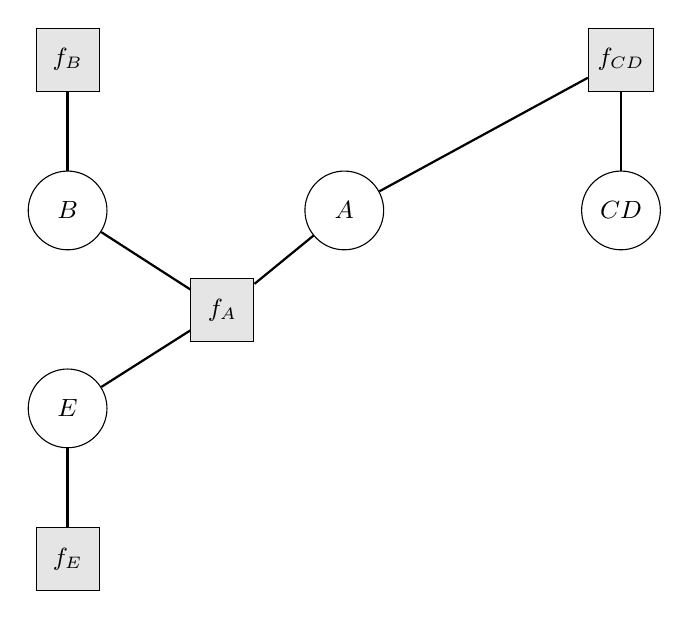
\begin{tikzpicture}[
  var/.style={circle, draw, minimum size=10mm, font=\small},
  fac/.style={rectangle, draw, fill=gray!20, minimum size=8mm, font=\small},
  edge/.style={thick},
  node distance=18mm
]
  \node[var] (B) {$B$};
  \node[var, right=25mm of B] (A) {$A$};
  \node[var, below=15mm of B] (E) {$E$};
  \node[var, right=25mm of A] (CD) {$CD$};
  \node[fac, above=10mm of B] (fB) {$f_B$};
  \node[fac, below=10mm of E] (fE) {$f_E$};
  \node[fac, below right=5mm and 12mm of B] (fA) {$f_A$};
  \node[fac, above=10mm of CD] (fCD) {$f_{CD}$};
  \draw[edge] (B) -- (fB);
  \draw[edge] (E) -- (fE);
  \draw[edge] (B) -- (fA);
  \draw[edge] (E) -- (fA);
  \draw[edge] (A) -- (fA);
  \draw[edge] (A) -- (fCD);
  \draw[edge] (CD) -- (fCD);
\end{tikzpicture}
\end{center}

\subsection{Credal Factors (Extreme Points)}

\paragraph{$f_B$: $K(B)$.} $v_1 = [0.80, 0.20]$, \; $v_2 = [0.90, 0.10]$.

\paragraph{$f_E$: $K(E)$.} $v_1 = [0.90, 0.10]$, \; $v_2 = [0.95, 0.05]$.

\paragraph{$f_A$: $K(A \mid B, E)$.} 4 parent configs, 2 vertices each:

\begin{center}
\begin{tabular}{llcc}
\toprule
\textbf{Config} & \textbf{Vtx} & $P(A{=}0)$ & $P(A{=}1)$ \\
\midrule
$B{=}0, E{=}0$ & $v_1$ & 0.9556 & 0.0444 \\
$B{=}0, E{=}0$ & $v_2$ & 1.0000 & 0.0000 \\
\midrule
$B{=}1, E{=}0$ & $v_1$ & 0.0000 & 1.0000 \\
$B{=}1, E{=}0$ & $v_2$ & 1.0000 & 0.0000 \\
\midrule
$B{=}0, E{=}1$ & $v_1$ & 0.0000 & 1.0000 \\
$B{=}0, E{=}1$ & $v_2$ & 1.0000 & 0.0000 \\
\midrule
$B{=}1, E{=}1$ & $v_1$ & 0.0000 & 1.0000 \\
$B{=}1, E{=}1$ & $v_2$ & 1.0000 & 0.0000 \\
\bottomrule
\end{tabular}
\end{center}

\paragraph{$f_{CD}$: $K(CD \mid A)$.} $A{=}0$: 4 vertices; $A{=}1$: 11 vertices (see companion documents for full listing).

\subsection{Query 1: $P(B{=}1)$, No Evidence}

\paragraph{Step 1: Initialization.}
Each distribution is set to the center (average) of its credal set:
\begin{align*}
  P(B) &= \tfrac{1}{2}([0.80, 0.20] + [0.90, 0.10]) = [0.85,\; 0.15], \\
  P(E) &= \tfrac{1}{2}([0.90, 0.10] + [0.95, 0.05]) = [0.925,\; 0.075], \\
  P(A \mid B{=}0, E{=}0) &= \tfrac{1}{2}([0.9556, 0.0444] + [1.0, 0.0]) = [0.9778,\; 0.0222].
\end{align*}
(Other parent configs for $A$ are similarly averaged.)

\paragraph{Step 2: Initial evaluation.}
Run VE with these fixed distributions:
\[
  P(B{=}1) = 0.1500 \quad \text{(the center value for $B$).}
\]

\paragraph{Step 3: Coordinate descent (sense = $\min$).}

\textbf{Iteration 0:}

\emph{Try variable $B$, config $()$:}
\begin{itemize}
  \item Set $P(B) = v_1 = [0.80, 0.20]$, run VE: $P(B{=}1) = 0.2000$.
        Worse than $0.1500$ $\to$ reject.
  \item Set $P(B) = v_2 = [0.90, 0.10]$, run VE: $P(B{=}1) = 0.1000$.
        Better $\to$ \textbf{accept}. Update incumbent: $p^* = 0.1000$.
\end{itemize}

\emph{Try variable $E$, config $()$:}
\begin{itemize}
  \item $v_1 = [0.90, 0.10]$: VE gives $P(B{=}1) = 0.1000$. No improvement.
  \item $v_2 = [0.95, 0.05]$: VE gives $P(B{=}1) = 0.1000$. No improvement.
\end{itemize}

Since $B$ is a root node, $P(B)$ directly determines $P(B{=}1)$ regardless of
other distributions. The algorithm correctly identifies $v_2 = [0.90, 0.10]$ as the
minimizer in one iteration.

\emph{Other variables ($A$, $CD$)} have no effect on $P(B{=}1)$ after $B$'s vertex is fixed.

\textbf{Iteration 1:} No improvement found $\to$ converged.

\textbf{Result (min):} $\underline{P}(B{=}1) = 0.1000$.

\paragraph{Coordinate descent (sense = $\max$).}
Analogous: selecting $v_1 = [0.80, 0.20]$ gives $\overline{P}(B{=}1) = 0.2000$.
Converges in 1 iteration.

\paragraph{Final result:}
\[
  \boxed{P(B{=}1) \in [0.1000,\; 0.2000].}
\]

\subsection{Query 2: $P(A{=}1 \mid B{=}0, E{=}0)$}

\paragraph{Initialization.}
With evidence $B{=}0, E{=}0$, the only relevant parent config for $A$ is $(B{=}0, E{=}0)$.
The initial center distribution is:
\[
  P(A \mid B{=}0, E{=}0) = [0.9778,\; 0.0222].
\]

\paragraph{Initial evaluation.}
VE with fixed distributions and evidence gives $P(A{=}1 \mid B{=}0, E{=}0) = 0.0222$.

\paragraph{Coordinate descent (sense = $\min$).}

\emph{Try $A$, config $(B{=}0, E{=}0)$:}
\begin{itemize}
  \item $v_1 = [0.9556, 0.0444]$: VE gives $P(A{=}1) = 0.0444$. Worse $\to$ reject.
  \item $v_2 = [1.0000, 0.0000]$: VE gives $P(A{=}1) = 0.0000$. Better $\to$ \textbf{accept}.
\end{itemize}

Converged: $\underline{P}(A{=}1 \mid B{=}0, E{=}0) = 0.0000$.

\paragraph{Coordinate descent (sense = $\max$).}

\emph{Try $A$, config $(B{=}0, E{=}0)$:}
\begin{itemize}
  \item $v_1 = [0.9556, 0.0444]$: $P(A{=}1) = 0.0444$. Better $\to$ \textbf{accept}.
  \item $v_2 = [1.0, 0.0]$: $P(A{=}1) = 0.0000$. Worse $\to$ reject.
\end{itemize}

Converged: $\overline{P}(A{=}1 \mid B{=}0, E{=}0) = 0.0444$.

\paragraph{Final result:}
\[
  \boxed{P(A{=}1 \mid B{=}0, E{=}0) \in [0.0000,\; 0.0444].}
\]

Both results match exact VE, confirming that ApproxLP finds the global optimum on this network.

\section{Properties}

\paragraph{Inner bounds.}
ApproxLP produces \emph{inner} bounds: the returned interval $[\underline{P}, \overline{P}]$
is guaranteed to satisfy $\underline{P}_{\mathrm{true}} \leq \underline{P}$ and
$\overline{P} \leq \overline{P}_{\mathrm{true}}$. This is because coordinate descent
explores a subset of the feasible extreme point combinations.

\paragraph{Monotonic convergence.}
Each iteration either improves the objective or stops. The objective is bounded, so
convergence is guaranteed in a finite number of steps.

\paragraph{Local optima.}
Coordinate descent may get stuck at a local optimum: the current combination of vertices
may be locally optimal (no single vertex swap improves the objective) but globally
suboptimal (a simultaneous swap of multiple vertices would improve it). In practice,
this is rarely an issue for small to medium networks.

\paragraph{Speed.}
Each VE evaluation operates on a \emph{precise} Bayesian network (single distributions,
no sets of functions), which is orders of magnitude faster than credal VE. For the alarm
network: ApproxLP takes $0.007$\,s vs.\ credal VE's $3.76$\,s---a $500\times$ speedup.

\section{Comparison with Other Methods}

\begin{center}
\begin{tabular}{lccccc}
\toprule
\textbf{Property} & \textbf{Exact VE} & \textbf{$\varepsilon$-VE} & \textbf{CTE}
  & \textbf{IBP} & \textbf{ApproxLP} \\
\midrule
Exact & Yes & No & Yes & No & No \\
Bound type & Tight & Outer & Tight & Outer & Inner \\
All marginals & No & No & Yes & No & No \\
Multi-valued & Yes & Yes & Yes & Yes & Yes \\
Speed (alarm) & 3.76\,s & 0.009\,s & 50\,s & 0.01\,s & 0.007\,s \\
\bottomrule
\end{tabular}
\end{center}

ApproxLP and IBP produce complementary bounds: ApproxLP's inner bounds sit inside the
true interval, while IBP's outer bounds contain it. Together they can bracket the true
interval from both sides.

\section{Complexity}

Each coordinate descent iteration visits all variables, all parent configs, and all
extreme points. For each vertex tried, a full VE is run on a precise BN.

\begin{itemize}
  \item \textbf{Per VE evaluation}: $O(n \cdot k^{w^*})$ where $n$ is the number of
        variables, $k$ the max domain size, and $w^*$ the treewidth.
  \item \textbf{Per iteration}: $O\bigl(\sum_i \sum_{\pi} |\mathrm{ext}\,K(X_i \mid \pi)|\bigr)
        \times O(n \cdot k^{w^*})$ VE evaluations.
  \item \textbf{Total}: $O(T \cdot V_{\mathrm{total}} \cdot n \cdot k^{w^*})$ where $T$ is
        the number of iterations and $V_{\mathrm{total}}$ is the total number of extreme
        points across all credal sets.
\end{itemize}

In practice, $T$ is typically 2--5 (fast convergence), making ApproxLP very efficient.

\section{References}

\begin{enumerate}
\item A.\ Antonucci, C.P.\ de Campos, D.\ Huber, M.\ Zaffalon. Approximating credal
      network inferences by linear programming. \emph{ECSQARU}, 7958:13--25, 2013.
\item A.\ Antonucci, C.P.\ de Campos, D.\ Huber, M.\ Zaffalon. Approximate credal
      network updating by linear programming with applications to decision making.
      \emph{IJAR}, 58:25--38, 2015.
\item C.P.\ de Campos, F.G.\ Cozman. Inference in credal networks using multilinear
      programming. \emph{STAIRS}, 2004.
\item A.M.\ Lukatskii, D.V.\ Shapot. Problems in multilinear programming.
      \emph{Comp.\ Math.\ Math.\ Phys.}, 41:638--648, 2000.
\item D.D.\ Mau\'a, F.G.\ Cozman. Thirty years of credal networks. \emph{IJAR},
      126:133--157, 2020.
\end{enumerate}

\end{document}
